% Options for packages loaded elsewhere
\PassOptionsToPackage{unicode}{hyperref}
\PassOptionsToPackage{hyphens}{url}
\documentclass[
  10pt,
  a4paper,
]{article}
\usepackage{xcolor}
\usepackage[margin=22mm]{geometry}
\usepackage{amsmath,amssymb}
\setcounter{secnumdepth}{-\maxdimen} % remove section numbering
\usepackage{iftex}
\ifPDFTeX
  \usepackage[T1]{fontenc}
  \usepackage[utf8]{inputenc}
  \usepackage{textcomp} % provide euro and other symbols
\else % if luatex or xetex
  \usepackage{unicode-math} % this also loads fontspec
  \defaultfontfeatures{Scale=MatchLowercase}
  \defaultfontfeatures[\rmfamily]{Ligatures=TeX,Scale=1}
\fi
\usepackage{lmodern}
\ifPDFTeX\else
  % xetex/luatex font selection
\fi
% Use upquote if available, for straight quotes in verbatim environments
\IfFileExists{upquote.sty}{\usepackage{upquote}}{}
\IfFileExists{microtype.sty}{% use microtype if available
  \usepackage[]{microtype}
  \UseMicrotypeSet[protrusion]{basicmath} % disable protrusion for tt fonts
}{}
\makeatletter
\@ifundefined{KOMAClassName}{% if non-KOMA class
  \IfFileExists{parskip.sty}{%
    \usepackage{parskip}
  }{% else
    \setlength{\parindent}{0pt}
    \setlength{\parskip}{6pt plus 2pt minus 1pt}}
}{% if KOMA class
  \KOMAoptions{parskip=half}}
\makeatother
\usepackage{graphicx}
\makeatletter
\newsavebox\pandoc@box
\newcommand*\pandocbounded[1]{% scales image to fit in text height/width
  \sbox\pandoc@box{#1}%
  \Gscale@div\@tempa{\textheight}{\dimexpr\ht\pandoc@box+\dp\pandoc@box\relax}%
  \Gscale@div\@tempb{\linewidth}{\wd\pandoc@box}%
  \ifdim\@tempb\p@<\@tempa\p@\let\@tempa\@tempb\fi% select the smaller of both
  \ifdim\@tempa\p@<\p@\scalebox{\@tempa}{\usebox\pandoc@box}%
  \else\usebox{\pandoc@box}%
  \fi%
}
% Set default figure placement to htbp
\def\fps@figure{htbp}
\makeatother
\setlength{\emergencystretch}{3em} % prevent overfull lines
\providecommand{\tightlist}{%
  \setlength{\itemsep}{0pt}\setlength{\parskip}{0pt}}
\usepackage{mathrsfs}
\usepackage{mathtools}
\usepackage{xurl}
\emergencystretch=3em
\setcounter{tocdepth}{1}
\newcommand{\Beta}{\mathrm{B}}
\DeclareUnicodeCharacter{00B2}{\ensuremath{^2}}
\DeclareUnicodeCharacter{00B1}{\ensuremath{\pm}}
\DeclareUnicodeCharacter{00D7}{\ensuremath{\times}}
\DeclareUnicodeCharacter{2192}{\ensuremath{\to}}
\DeclareUnicodeCharacter{21D2}{\ensuremath{\Rightarrow}}
\DeclareUnicodeCharacter{21A6}{\ensuremath{\mapsto}}
\DeclareUnicodeCharacter{2208}{\ensuremath{\in}}
\DeclareUnicodeCharacter{2209}{\ensuremath{\notin}}
\DeclareUnicodeCharacter{2212}{\ensuremath{-}}
\DeclareUnicodeCharacter{2227}{\ensuremath{\wedge}}
\DeclareUnicodeCharacter{2228}{\ensuremath{\vee}}
\DeclareUnicodeCharacter{2260}{\ensuremath{\ne}}
\DeclareUnicodeCharacter{2264}{\ensuremath{\le}}
\DeclareUnicodeCharacter{2265}{\ensuremath{\ge}}
\DeclareUnicodeCharacter{2297}{\ensuremath{\otimes}}
\DeclareUnicodeCharacter{00B3}{\ensuremath{^3}}
\DeclareUnicodeCharacter{2074}{\ensuremath{^4}}
\DeclareUnicodeCharacter{2076}{\ensuremath{^6}}
\DeclareUnicodeCharacter{03BB}{\ensuremath{\lambda}}
\DeclareUnicodeCharacter{03BC}{\ensuremath{\mu}}
\DeclareUnicodeCharacter{03B5}{\ensuremath{\epsilon}}
\DeclareUnicodeCharacter{03C4}{\ensuremath{\tau}}
\DeclareUnicodeCharacter{03A6}{\ensuremath{\Phi}}
\DeclareUnicodeCharacter{03B1}{\ensuremath{\alpha}}
\DeclareUnicodeCharacter{03C3}{\ensuremath{\sigma}}
\DeclareUnicodeCharacter{03B4}{\ensuremath{\delta}}
\DeclareUnicodeCharacter{03C0}{\ensuremath{\pi}}
\DeclareUnicodeCharacter{039B}{\ensuremath{\Lambda}}
\DeclareUnicodeCharacter{2202}{\ensuremath{\partial}}
\DeclareUnicodeCharacter{0393}{\ensuremath{\Gamma}}
\DeclareUnicodeCharacter{2205}{\ensuremath{\varnothing}}
\DeclareUnicodeCharacter{221E}{\ensuremath{\infty}}
\DeclareUnicodeCharacter{2200}{\ensuremath{\forall}}
\DeclareUnicodeCharacter{00B9}{\ensuremath{^1}}
\DeclareUnicodeCharacter{00B0}{\ensuremath{{}^\circ}}
\DeclareUnicodeCharacter{211D}{\ensuremath{\mathbb{R}}}
\usepackage{bookmark}
\IfFileExists{xurl.sty}{\usepackage{xurl}}{} % add URL line breaks if available
\urlstyle{same}
\hypersetup{
  hidelinks,
  pdfcreator={LaTeX via pandoc}}

\author{}
\date{}

\begin{document}

{
\setcounter{tocdepth}{3}
\tableofcontents
}
\section{The original zeta function, faithful theta recovery, and the
heat return
defect}\label{the-original-zeta-function-faithful-theta-recovery-and-the-heat-return-defect}

This calculation retains the original meromorphic Riemann zeta function,
its full multiplier, the supported-zero contribution, and every lower
support coefficient. It reconstructs the theta input explicitly and
calculates the obstruction to realizing the source heat family by
another input in the same theta domain. The obstruction is then mapped
isomorphically to specified meromorphic principal parts. No assertion of
RH is used.

\subsection{1. Original carrier and exact analytic
domain}\label{original-carrier-and-exact-analytic-domain}

Let \(L\) be a finite bounded distributive lattice with distinct bottom
and top. The carrier is \[
G_L(A)=\{(a,1_L):a\in A\}\cup\{z_\lambda=(0,\lambda):\lambda\ne1_L\},
\quad e_L=(0,1_L),\quad\tau_L=(0,0_L).
\tag{TF1}
\] Addition uses amplitude addition and support join; multiplication
uses amplitude multiplication and support meet. In the two-support
integer subcarrier the principal ideals are \[
(\tau)=\{\tau\}\subsetneq(e)=\{\tau,e\}\subsetneq
(p)=\{\tau\}\cup(p\mathbb Z)^\bullet.
\tag{TF2}
\] Each is prime: an unsupported product has an unsupported factor; a
supported product has amplitude zero only if one integer factor has
amplitude zero; and divisibility by an ordinary prime is tested on the
amplitudes. This retains the prime supported zero. It does not identify
it with the unsupported element. The complete lattice and adelic carrier
maps are the retained SZW1--13 proof in
\texttt{SUPPORTED\_\allowbreak{}ZERO\_\allowbreak{}PRIME\_\allowbreak{}WEIL\_\allowbreak{}DERIVATION.\allowbreak{}md}; the present domain
is its global fixed-sector carrier, not the larger carrier with
nonconstant proper adelic strata.

Use exactly \[
\mathcal F_L=\mathcal S_{\rm ev}(\mathbb R)\oplus
\bigoplus_{\lambda\ne1_L}\mathbb C\delta_\lambda,
\qquad F=(\phi,(c_\lambda)),
\qquad \widehat\phi(y)=\int_{\mathbb R}\phi(x)e^{-2\pi ixy}\,dx.
\tag{TF3}
\] The point-functions \(\delta_\lambda\) retain separate coefficients.
They are not Dirac distributions on the real line. For \(x>0\), put \[
a=\phi(0),\quad b=\int_{\mathbb R}\phi(x)\,dx,\quad
\Theta_e\phi(x)=\sum_{n\in\mathbb Z}\phi(nx),\quad
P\phi(x)=\sum_{n\ne0}\phi(nx).
\tag{TF4}
\] The labelled sum is
\(\Theta_e\phi(x)\,\mathbf e_{1_L}+\sum_{\lambda\ne1_L}c_\lambda\mathbf e_\lambda\),
where the \(\mathbf e_\lambda\) are independent coordinates in
\(\mathbb C^L\). Its top coordinate includes the supported zero once. On
compact positive \(x\)-intervals every derivative of the sums converges
absolutely by a sufficiently high Schwartz bound. Poisson summation
gives \[
\Theta_e\phi(x)=x^{-1}\Theta_e\widehat\phi(x^{-1}),\qquad
P\phi(x)=x^{-1}P\widehat\phi(x^{-1})+b/x-a.
\tag{TF5}
\] For each lower coordinate the raw Fourier convention fixes
\(c_\lambda\); its Poisson defect is exactly \(c_\lambda(1-x^{-1})\).
These distinct defects must not be replaced by their possibly vanishing
scalar sum.

\subsection{2. Original zeta in the Mellin
calculation}\label{original-zeta-in-the-mellin-calculation}

For \(\Re s>1\), absolute convergence and the substitution \(y=nx\) give
\[
Z_\phi(s)=\int_0^\infty P\phi(x)x^{s-1}\,dx
=2\zeta(s)\mathcal M\phi(s),\qquad
\mathcal M\phi(s)=\int_0^\infty\phi(x)x^{s-1}\,dx.
\tag{TF6}
\] Here \(\zeta(s)=\sum_{n\ge1}n^{-s}\) on that half-plane. The Mellin
transform \(\mathcal M\phi\) is holomorphic on \(\Re s>0\), because
\(\phi\) is bounded near zero and has arbitrarily high decay at
infinity; the same bounds with powers of \(\log x\) justify parameter
derivatives. Splitting TF6 at one and applying TF5 gives the exact
continuation \[
Z_\phi(s)=\int_1^\infty P\phi(x)x^{s-1}\,dx
+\int_1^\infty P\widehat\phi(x)x^{-s}\,dx
+\frac{b}{s-1}-\frac{a}{s}.
\tag{TF7}
\] Both integrals are entire, by the derivative versions of the Schwartz
bounds. The residues are \(b\) at one and \(-a\) at zero. Lower fixed
coefficients have two separate tail terms \(c_\lambda/s\) and
\(-c_\lambda/s\). Their meromorphic sum is zero, while each fixed
representation has its nonzero character distribution; SZW16--18 proves
both maps. We retain \((c_\lambda)\) alongside TF6--7.

For the original Gaussian \(\phi_{\rm G}(x)=e^{-\pi x^2}\), substitution
\(y=\pi x^2\) gives \[
\mathcal M\phi_{\rm G}(s)=\frac12\pi^{-s/2}\Gamma(s/2),\quad
Z_{\phi_{\rm G}}(s)=\pi^{-s/2}\Gamma(s/2)\zeta(s).
\tag{TF8}
\] Thus the Gaussian is a specified analytic input. TF1 alone does not
select this input, its measure, or the subsequent heat operation. Its
comparison to the original zeta is TF8 with every factor retained.

\subsection{3. The exact theta filter and its
inverse}\label{the-exact-theta-filter-and-its-inverse}

Define \[
w_\phi(u)=e^u\Theta_e\phi(e^{2u}),\qquad
\Phi_\phi(u)=\frac1{16}(D_u^2-1)w_\phi(u).
\tag{TF9}
\] For every derivative order \(j\) and \(A>0\), Schwartz estimates and
TF5 prove \[
D_u^j(w_\phi-ae^u)=O_{A,j}(e^{-Au})\quad(u\to+\infty),
\qquad
D_u^j(w_\phi-be^{-u})=O_{A,j}(e^{Au})\quad(u\to-\infty).
\tag{TF10}
\] Indeed differentiating a summand introduces powers of \(ne^{2u}\),
bounded by a higher Schwartz seminorm and a convergent inverse-power sum
in \(n\). This proves the first estimate; apply the same bound to
\(\widehat\phi\) in TF5 for the second. Since \(D_u^2-1\) annihilates
both exponential terms, \(\Phi_\phi\) and all its derivatives decrease
faster than every exponential at both ends.

The endpoint coefficients are exactly recoverable: \[
a=8\int_{\mathbb R}e^{-u}\Phi_\phi(u)\,du,
\qquad b=8\int_{\mathbb R}e^u\Phi_\phi(u)\,du.
\tag{TF11}
\] To prove this, differentiate the two Wronskians: \[
\big(e^{-u}(w_\phi'+w_\phi)\big)'=16e^{-u}\Phi_\phi,
\qquad
\big(e^u(w_\phi'-w_\phi)\big)'=16e^u\Phi_\phi.
\tag{TF12}
\] The first bracket has limits zero and \(2a\), and the second has
limits \(-2b\) and zero, at the negative and positive ends respectively.
TF10 proves each limit and absolute integrability. Integration gives
TF11.

The complete inverse at the theta level is \[
\begin{aligned}
w_\phi(u)
&=a e^u+16\int_u^\infty\sinh(v-u)\Phi_\phi(v)\,dv\\
&=8\int_{\mathbb R}e^{|u-v|}\Phi_\phi(v)\,dv.
\end{aligned}
\tag{TF13}
\] For the first expression, two differentiations give
\((D_u^2-1)w=16\Phi_\phi\). Its difference from the original \(w_\phi\)
is a homogeneous solution \(Ae^u+Be^{-u}\), decreasing faster than every
exponential as \(u\to+\infty\) by TF10 and the tail estimate. Both
constants are therefore zero. The second expression follows by inserting
TF11 and splitting its integral at \(u\). No endpoint coefficient has
been assigned by an arbitrary boundary choice.

The input itself is recovered without division at a zeta zero: \[
\Theta_e\phi(x)=x^{-1/2}w_\phi(\tfrac12\log x),\qquad
\phi(x)=\frac12\sum_{n\ge1}\mu(n)
\big(\Theta_e\phi(nx)-a\big),\quad x>0.
\tag{TF14}
\] Substituting TF4 gives \(\sum_{n,k\ge1}\mu(n)\phi(knx)\). Its
absolute sum is at most \(\sum_{m\ge1}d(m)|\phi(mx)|<\infty\) for fixed
\(x>0\), since \(d(m)\le m\) and Schwartz decay beats any fixed power.
Regrouping and \(\sum_{n\mid m}\mu(n)=\mathbf1_{m=1}\) prove TF14.
Evenness and the recovered \(a\) recover the other arguments.

Consequently the following is an explicit linear isomorphism onto its
image: \[
\mathcal F_L\longrightarrow
\{\Phi_\phi:\phi\in\mathcal S_{\rm ev}(\mathbb R)\}
\oplus\mathbb C^{L\setminus\{1_L\}},
\qquad F\longmapsto(\Phi_\phi,(c_\lambda)).
\tag{TF15}
\] It keeps every coordinate. The profile alone has kernel exactly the
lower coefficient space, so the corresponding sequence with that kernel
is split exact. On the restricted theta image the differential filter
has no further kernel, despite its two-dimensional kernel on
unrestricted smooth functions. The inverse is asserted on the displayed
image, not on every rapidly decreasing profile. The even domain is
essential: enlarging to all Schwartz functions would kill its odd part
in TF4.

\subsection{4. Every multiplier and the source heat
kernel}\label{every-multiplier-and-the-source-heat-kernel}

Set \(\kappa=2s-1\). For \(\Re s>1\), the function \(w_\phi-ae^u\)
satisfies \(\int_{\mathbb R}(w_\phi-ae^u)e^{\kappa u}du=Z_\phi(s)/2\).
At the positive end every boundary derivative decays faster than the
exponential weight. At the negative end its terms have exponents
\(2s-2\) and \(2s\), so both boundary terms also vanish. Two
integrations by parts in TF9 therefore prove \[
4\int_{\mathbb R}\Phi_\phi(u)e^{(2s-1)u}\,du
=\frac12s(s-1)Z_\phi(s)
=s(s-1)\zeta(s)\mathcal M\phi(s).
\tag{TF16}
\] The integral is entire. Its endpoint values are \(a/2\) and \(b/2\),
directly from TF11; the same values follow by retaining the residues in
TF7.

For the Gaussian, differentiate each \(e^{u-A}\), where
\(A=\pi n^2e^{4u}\). Its image under \(D_u^2-1\) is
\(8(2A^2-3A)e^{u-A}\). Counting both \(n\) and \(-n\) and the factor
\(1/16\) gives \[
\Phi_{\rm G}(u)=\sum_{n\ge1}
\big(2\pi^2n^4e^{9u}-3\pi n^2e^{5u}\big)e^{-\pi n^2e^{4u}}.
\tag{TF17}
\] Poisson summation for the self-Fourier Gaussian makes \(w_{\rm G}\)
and hence \(\Phi_{\rm G}\) even. For \(u\ge0\), every summand in TF17 is
positive, since \(2\pi n^2e^{4u}>3\). The series and derivatives have
double-exponential decay at both ends. TF17 is precisely the original
Rodgers--Tao density, with its original variable \(u\).

Keep the multiplier itself visible: \[
C(s)=\frac12s(s-1)\pi^{-s/2}\Gamma(s/2),\qquad
4\int_{\mathbb R}\Phi_{\rm G}(u)e^{(2s-1)u}\,du=C(s)\zeta(s).
\tag{TF18}
\] For the original source convention \[
H_t(Z)=\int_0^\infty e^{tu^2}\Phi_{\rm G}(u)\cos(Zu)\,du,
\qquad s=\frac12+\frac{iZ}{2},
\] \[
H_0(Z)=\frac18 C(s)\zeta(s),\qquad
\zeta_t(s):=
\frac{8\int_0^\infty e^{tu^2}\Phi_{\rm G}(u)
\cosh((2s-1)u)\,du}
{\frac12s(s-1)\pi^{-s/2}\Gamma(s/2)},\qquad \zeta_0=\zeta.
\tag{TF19}
\] This is a specified meromorphic deformation of the original zeta, not
a claim of an Euler product at nonzero time. All complex \((t,s)\)
derivatives of the numerator converge locally uniformly by the
double-exponential bounds. The original source satisfies
\(\partial_tH_t=-\partial_Z^2H_t\); applying the displayed coordinate
and multiplier gives \[
\begin{aligned}
\partial_t\zeta_t&=\frac14\bigg[
\zeta_t''+2\left(\frac1s+\frac1{s-1}-\frac{\log\pi}{2}
+\frac12\psi(s/2)\right)\zeta_t'\\
&\quad+\bigg\{-\frac1{s^2}-\frac1{(s-1)^2}+\frac14\psi_1(s/2)\\
&\qquad
+\left(\frac1s+\frac1{s-1}-\frac{\log\pi}{2}
+\frac12\psi(s/2)\right)^2\bigg\}\zeta_t\bigg].
\end{aligned}
\tag{TF20}
\] Here \(\psi=\Gamma'/\Gamma\) and \(\psi_1=\psi'\). Differentiating
the full product \(C\zeta_t\) proves every term. Its globally valid
interpretation is a meromorphic identity. The companion
\texttt{FAITHFUL\_\allowbreak{}UNCOMPLETED\_\allowbreak{}ZETA\_\allowbreak{}HEAT.\allowbreak{}md} proves the local
fractional-module isomorphisms, every exceptional-point jet, the signed
full divisor, and the trace domains; these remain part of the return,
not optional factors to drop.

\subsection{5. The original-domain obstruction in original zeta
coordinates}\label{the-original-domain-obstruction-in-original-zeta-coordinates}

Let \(U=\{s:0<\Re s<1\}\). The actual \(C\) is holomorphic and nowhere
zero on \(U\). Dividing TF16 by this specified multiplier, on this
specified domain, proves \[
\frac{4\int_{\mathbb R}\Phi_\phi(u)e^{(2s-1)u}\,du}{C(s)}
=\zeta(s)\frac{2\pi^{s/2}}{\Gamma(s/2)}\mathcal M\phi(s).
\tag{TF21}
\] Every original theta input therefore retains every original
nontrivial zero with at least its full multiplicity. This is a
divisibility assertion for the original \(\zeta\), not a consequence of
RH.

For each fixed \(s\in U\), substitution \(u=v/\sqrt T\) in TF19 proves
\[
\lim_{T\to\infty}\sqrt T\,\zeta_{-T}(s)
=\frac{4\sqrt\pi\,\Phi_{\rm G}(0)}
{\frac12s(s-1)\pi^{-s/2}\Gamma(s/2)}\ne0.
\tag{TF22}
\] Indeed for \(T\ge1\) the rescaled integrand is dominated by a
constant times \(e^{-v^2+|2s-1|v}\). The limiting Gaussian integral is
\(\sqrt\pi/2\), and TF17 gives \(\Phi_{\rm G}(0)>0\). Dominated
convergence supplies the exact coefficient.

Fix an original nontrivial zero \(\rho\), of multiplicity \(m_\rho\).
The entire function \(t\mapsto\zeta_t(\rho)\) is not identically zero by
TF22, and vanishes at time zero. It therefore has a finite vanishing
order \(n_\rho\ge1\): \[
\zeta_t(\rho)=t^{n_\rho}u_\rho(t),\qquad
u_\rho(0)=
\frac{(C\zeta)^{(2n_\rho)}(\rho)}
{C(\rho)4^{n_\rho}n_\rho!}\ne0.
\tag{TF23}
\] The Taylor identity follows from TF20 before product division, or
directly from differentiating TF19. A sufficiently small disk has
\(u_\rho(t)\ne0\). For every nonzero time in that disk, \(\zeta_t\)
cannot be the TF21 receiver of any original even Schwartz theta input.
One fixed zero gives this assertion; no uniform radius over all zeros is
claimed. The existence of nontrivial zeros is also independent of RH, as
the original zero-counting theorem gives; here each assertion is proved
for every such zero individually.

The defect is the actual object \[
\Omega_t=[\zeta_t|_U]\in\mathcal O(U)/(\zeta),\qquad
\Omega_0=0,\quad\Omega_t\ne0\text{ for all sufficiently small }t\ne0.
\tag{TF24}
\] Let \(A_\rho=\mathbb C[\epsilon_\rho]/(\epsilon_\rho^{m_\rho})\).
Taylor restriction gives an isomorphism \[
\mathcal O(U)/(\zeta)\longrightarrow
\prod_\rho A_\rho,\qquad
[f]\longmapsto\left(
\sum_{j=0}^{m_\rho-1}\frac{f^{(j)}(\rho)}{j!}\epsilon_\rho^j
\right)_\rho.
\tag{TF25}
\] The kernel is exactly \(\zeta\mathcal O(U)\), by removable division
at each zero. Here is a constructive surjectivity proof retaining
arbitrary jets and their multiplicities. The entire function
\(E=C\zeta\) has exactly these zeros, none at zero. For prescribed
polynomial jets \(p_\rho\), take the principal part \(Q_\rho\) of
\(p_\rho(s-\rho)/E(s)\). Enumerate the discrete zero set by
\(|\rho_j|\to\infty\), choose \(R_j<|\rho_j|\) tending to infinity, and
subtract a Taylor polynomial \(T_j\) of \(Q_{\rho_j}\) such that
\(\sup_{|s|\le R_j}|Q_{\rho_j}-T_j|<2^{-j}\). The series of differences
converges uniformly on compact sets away from its poles and has the
prescribed principal parts. Multiplication by \(E\) yields an entire
function with precisely the prescribed jets. Restriction to \(U\) proves
surjectivity. This use of \(E=C\zeta\) retains its full multiplier and
is only an interpolation construction, not a replacement for the
original defect TF24.

The local time coefficients of TF24, including all lower jets, are \[
[t^n]\Omega_t\big|_\rho
=\sum_{j=0}^{m_\rho-1}\frac{1}{4^n n!j!}
\left.\partial_s^j\left(C(s)^{-1}
\partial_s^{2n}(C(s)\zeta(s))\right)\right|_{s=\rho}
\epsilon_\rho^j.
\tag{TF26}
\] At a multiple zero write
\(\zeta(\rho+\epsilon)=\epsilon^m v_\rho(\epsilon)\), \(v_\rho(0)\ne0\).
The complete first-order expression is \[
\frac14\left[\zeta''+2\frac{C'}C\zeta'
+\frac{C''}C\zeta\right]_\rho
=\frac{m(m-1)}4v_\rho(0)\epsilon^{m-2}
+\text{higher powers of }\epsilon\ne0\quad(m\ge2).
\tag{TF27}
\] Both lower-order multiplier terms remain in the left side. They
cannot cancel its displayed leading term, since their orders are at
least \(m-1\) and \(m\). Thus full jet departure occurs already at first
heat order at every multiple zero, even when its value departure TF23
occurs later.

\subsection{6. The meromorphic space exposed by the
defect}\label{the-meromorphic-space-exposed-by-the-defect}

The forced candidate Mellin transform for returning TF19 to TF16 is \[
\mathcal M_t(s)=
\frac{\pi^{-s/2}\Gamma(s/2)}2\frac{\zeta_t(s)}{\zeta(s)},
\qquad s\in U.
\tag{TF28}
\] Keep the prefactor \(\gamma_\infty(s)/2=\pi^{-s/2}\Gamma(s/2)/2\),
which is holomorphic and nowhere zero on \(U\). Let \(\mathcal P_\zeta\)
be the vector space of all families of principal parts at the original
zeros, with pole order at \(\rho\) at most \(m_\rho\). The map \[
\mathcal O(U)/(\zeta)\longrightarrow\mathcal P_\zeta,
\qquad [f]\longmapsto
\left(\operatorname{pp}_\rho
\frac{\pi^{-s/2}\Gamma(s/2)f(s)}{2\zeta(s)}\right)_\rho
\tag{TF29}
\] is a linear isomorphism. Locally multiplication by
\(\gamma_\infty/2\) and the nonvanishing unit in
\(\zeta=(s-\rho)^m v_\rho\) is invertible on every length-\(m\) jet.
This proves the local statement and the kernel; TF25 supplies all
prescribed local jets simultaneously and proves global surjectivity.
This is a vector-space isomorphism; no artificial multiplication on
principal parts is assumed.

In particular the heat defect has an exact meromorphic representative,
TF28, whose simple-zero residue is \[
\operatorname{Res}_{s=\rho}\mathcal M_t(s)
=\frac{\pi^{-\rho/2}\Gamma(\rho/2)}2
\frac{\zeta_t(\rho)}{\zeta'(\rho)}\quad(m_\rho=1).
\tag{TF30}
\] For multiplicity \(m\), writing \(\zeta(\rho+h)=h^m v_\rho(h)\) gives
all its principal coefficients by \[
\operatorname{pp}_\rho\mathcal M_t
=\sum_{j=0}^{m-1}\frac{h^{j-m}}{j!}
\left.\partial_h^j
\left(\frac{\pi^{-(\rho+h)/2}\Gamma((\rho+h)/2)}{2v_\rho(h)}
\zeta_t(\rho+h)\right)\right|_{h=0}.
\tag{TF31}
\] Every multiplier, orientation and coefficient is retained. TF28--31
define the enlarged meromorphic Mellin data exposed by the obstruction.
They do not assert that these data are the Mellin transform of an
original Schwartz function. That would contradict TF23. A zero class in
TF24 alone also does not characterize the theta image: set
\(f(s)=\zeta(s)/(s-2)\in\zeta\mathcal O(U)\). If it were the TF21
receiver of some \(\phi\), its product \(C(s)f(s)=C(s)\zeta(s)/(s-2)\)
would equal the entire integral in TF16. Analytic continuation
contradicts this because that product has a genuine pole at two:
\(C(2)\zeta(2)>0\). This uses the actual multiplication map into the
entire target. Multiplication by the explicit unit \(C|_U\) carries the
original heat defect to the completed heat defect as an invertible
module map, not as an algebra homomorphism; it does not enlarge the
original domain silently.

All operations TF24--31 act on the top analytic coordinate and carry
each unchanged \(c_\lambda\) separately. Forgetting those coefficients
has exactly the kernel in TF15. There is no identification of \(e_L\)
with \(\tau_L\), and no assumption that cancellation of a scalar finite
part erases a support coordinate.

\subsection{7. Fourier, dilation, and the domain of heat
multiplication}\label{fourier-dilation-and-the-domain-of-heat-multiplication}

Poisson summation gives the exact intertwining formulas \[
\Phi_{\widehat\phi}(u)=\Phi_\phi(-u),\qquad
\Phi_{V(y)\phi}(u)=\sqrt y\,\Phi_\phi(u-\tfrac12\log y),
\quad (V(y)\phi)(x)=\phi(x/y),\quad y>0.
\tag{TF32}
\] For the first, TF5 makes \(w_{\widehat\phi}(u)=w_\phi(-u)\), and the
operator in TF9 commutes with reflection. For the second, direct
substitution gives
\(w_{V(y)\phi}(u)=\sqrt y\,w_\phi(u-\tfrac12\log y)\); apply the same
constant-coefficient operator. Every \(c_\lambda\) stays fixed.
Substitution in TF11 recovers \(a\mapsto a\) and \(b\mapsto yb\), the
original endpoint characters.

Let \(\mathscr E\) consist of smooth profiles whose every derivative
decreases faster than every exponential at both ends. For each complex
time define the actual domain and map \[
\mathscr E_t=\{\Psi\in\mathscr E:e^{tu^2}\Psi\in\mathscr E\},
\qquad \mathscr H_t:\mathscr E_t\longrightarrow\mathscr E_{-t},
\quad\Psi\longmapsto e^{tu^2}\Psi.
\tag{TF33}
\] This is a linear isomorphism with inverse \(\mathscr H_{-t}\), by
direct multiplication. The Gaussian profile TF17 belongs to every
\(\mathscr E_t\), by its double-exponential estimates. This does not
imply that every original Schwartz theta profile belongs to every such
domain.

To prove the distinction, choose an even smooth cutoff \(\chi\) which is
zero on \(|x|\le e\) and one on \(|x|\ge e^2\), and put \[
\phi_*(x)=\chi(x)e^{-(\log|x|)^{3/2}}
\tag{TF34}
\] outside the zero region, with value zero inside. This is even
Schwartz. Every tail derivative is a finite sum of powers of \(x^{-1}\)
and powers of \(\log|x|\) and its reciprocal square root, multiplied by
the displayed exponential; it therefore decreases faster than every
power of \(|x|\). Smoothness on the cutoff region is part of its
construction. For \(E=x\partial_x\) and \(v=\log x\ge4\), direct
differentiation gives \[
E(E+1)\phi_*(x)=
\left(\frac94v-\frac32\sqrt v-\frac3{4\sqrt v}\right)e^{-v^{3/2}}
\ge v e^{-v^{3/2}}.
\tag{TF35}
\] Subtracting \(v\), the remaining coefficient is positive at four and
has positive derivative thereafter. Direct differentiation of TF9 also
gives \(\Phi_\phi(u)=\frac14e^u E(E+1)\Theta_e\phi(e^{2u})\). For
\(u\ge2\), each nonzero integer term is in the region of TF35 and is
positive. Keeping the two terms \(n=\pm1\) proves \[
\Phi_{\phi_*}(u)\ge u\exp\big(u-(2u)^{3/2}\big).
\tag{TF36}
\] For every real \(t>0\), multiplying this lower bound by \(e^{tu^2}\)
makes it nonintegrable against every fixed real exponential weight. Thus
\(\Phi_{\phi_*}\in\mathscr E\) but \(\Phi_{\phi_*}\notin\mathscr E_t\).
TF33 is the exact partial-domain replacement; TF24 and TF28--31 give the
additional arithmetic-image defect even on the everywhere-defined
Gaussian orbit.

\subsection{8. Source scope and consequences for the existing
calculations}\label{source-scope-and-consequences-for-the-existing-calculations}

Rodgers and Tao's original author TeX, arXiv:1801.05914v5,
\texttt{fmp-\allowbreak{}template.\allowbreak{}tex}, equations \texttt{hoz}, \texttt{phidef},
\texttt{htdef}, supplies precisely TF17 and the original \(H_t,Z,t\)
convention in TF19. The author source was read at lines 64--148 for this
comparison; this is not a claim to have read that entire paper. The
archive and original member are retained privately, SHA256
\texttt{25b015c0\allowbreak{}fb151f16\allowbreak{}13247d82\allowbreak{}cf53a656\allowbreak{}1a320d4d\allowbreak{}ab2bb4f8\allowbreak{}09482e7c\allowbreak{}477a5817}.
The original source is
\href{https://arxiv.org/abs/1801.05914v5}{Rodgers--Tao, The de
Bruijn--Newman constant is non-negative}.

The preceding theta/Poisson map is SZW5--23, read directly in the
programme source, with its exact Connes original-author TeX provenance
retained there. The independently derived checks TRR1--18 in
\texttt{THETA\_\allowbreak{}RETURN\_\allowbreak{}OBSTRUCTION\_\allowbreak{}INDEPENDENT\_\allowbreak{}REVIEW.\allowbreak{}md} verify the
constants, inverse, quotient and all multiplicity jets. The present
proof adds the explicit original-zeta coordinates and meromorphic
principal-part receiver rather than replacing those factors by an
auxiliary function.

TF15 proves faithful recovery on the stated full labelled theta domain.
TF19--20 gives the original-zeta heat receiver and every derivative
correction. TF23--31 proves that the usual heat operation does not
preserve that theta domain, and calculates the space and all local
coefficients measuring its failure. Consequently earlier heat positivity
or trace calculations require their actual original-zeta and support
receiving maps; they cannot be promoted to an operation on the unchanged
base merely from the initial Gaussian identity. Neither completion nor
this obstruction assumes, proves, or disproves RH.

\subsection{9. Exact comparison with the retained prime-boundary
receiver}\label{exact-comparison-with-the-retained-prime-boundary-receiver}

The complete companion proof
\href{https://github.com/KokunoYumeto/zeta-function-research-reader/blob/ec73ac350d0cda3d95c0bd1361bede33166b4d34/workbenches/splitzero-tandem/continuations/20260923-original-zeta-return/NOTE.tex}{FR1--38,
Original zeta, the theta source, and a faithful prime-boundary receiver}
was read in full for this comparison. The following calculation retains
its two prime-boundary coordinates and proves the precise map to TF9.
Its human sources remain Meyer, arXiv:math/0412277v3; Connes,
arXiv:math/9811068v1, Section III; and Connes--Consani,
arXiv:2207.10419v1, with the exact locators and reading scope in FR.
This is a comparison of those specified programme receivers, not a claim
to have reread those entire author sources here.

Write \(H=\mathcal S_{\rm ev}(\mathbb R)\),
\(m(\phi)=(\phi(0),\int_{\mathbb R}\phi)\), \(H_0=\ker m\), and retain
the nonzero-index operator \(\Theta\phi(x)=2\sum_{n\ge1}\phi(nx)\),
unlike the all-integer theta in TF3. Put \(D_x=-x\partial_x\) and
\(L_x=D_x(D_x-1)=x^2\partial_x^2+2x\partial_x\). Then \[
\Theta_e\phi(x)=\phi(0)+\Theta\phi(x),\qquad
\Phi_\phi(u)=\frac{e^u}{4}\Theta L_x\phi(e^{2u}),\qquad
8\int_{\mathbb R}\Phi_\phi(u)e^{(2s-1)u}\,du
=\int_0^\infty\Theta L_x\phi(x)x^{s-1}\,dx.
\tag{TF37}
\] Indeed \((\partial_u^2-1)(e^u f(e^{2u}))=4e^u L_x f(e^{2u})\); the
constant theta term contributes \((\partial_u^2-1)(\phi(0)e^u)=0\),
whose recovery was proved in TF11. Differentiated theta convergence
proves commutation with \(L_x\), and \(x=e^{2u}\), \(du=dx/(2x)\),
proves the last integral with its factor eight. In particular the
companion \(A(s)\) is exactly \(2C(s)\), and its heat numerator
\(U_t(s)\) is exactly \(2C(s)\zeta_t(s)\). Its returned function \(z_t\)
is our \(\zeta_t\), with unchanged time and spatial coordinates. TF11
becomes precisely FR14:
\(8\int e^{-u}\Phi_\phi=\int\Theta L_x\phi(x)dx/x=\phi(0)\), and
\(8\int e^u\Phi_\phi=\int\Theta L_x\phi(x)dx=\int\phi\).

For completeness \(L_x:H\to H_0\) is bijective, with all domains
visible. For \(k\in H_0\) put \(v(x)=-\int_x^\infty k(t)dt/t\), then
\(\phi(x)=-x^{-1}\int_x^\infty v(t)dt\). Since \(k(0)=0\) and \(k\) is
smooth and even, \(v\) extends evenly and smoothly at zero and is
Schwartz. Integration by parts gives
\(\int_0^\infty v=-\int_0^\infty k=0\). Hence
\(\phi=x^{-1}\int_0^xv(t)dt\) extends smoothly and evenly at zero; its
tail formula proves rapid decrease. Differentiation gives \(xv'=k\),
\((x\phi)'=v\), and therefore \(L_x\phi=k\). Conversely \(L_x\phi\) has
value zero at zero and integral zero by its derivative form. Its
homogeneous solutions on \(x>0\) are \(a+b/x\); only the zero one
belongs to \(H\). This proves bijectivity.

Let \(R=\mathbb C[\mathbb Q_{>0}^{\times}]\), with basis \(t_a\),
augmentation ideal \(I\), and \[
M_0=\ker(\operatorname{aug}\otimes m:R\otimes H\to\mathbb C^2),
\quad Q_0=M_0/IM_0,\quad
\mathcal B=\bigoplus_p\mathbb C\ell_p\otimes\mathbb C^2.
\tag{TF38}
\] All tensor expressions are finite sums. The moment lifts
\((1-2\pi x^2)e^{-\pi x^2}\) and \(2\pi x^2e^{-\pi x^2}\) have moments
\((1,0)\) and \((0,1)\). They give
\(M_0=(R\otimes H_0)\oplus(I\otimes\mathbb C^2)\), and hence
\(Q_0=H_0\oplus(I/I^2)\otimes\mathbb C^2\). The map
\(t_a-1\mapsto\sum_pv_p(a)\ell_p\) identifies \(I/I^2\) with
\(\bigoplus_p\mathbb C\ell_p\): the identity for \(t_{ab}-1\) proves
spanning, including inverse primes, while the derivations
\(\partial_p(t_a)=v_p(a)\) vanish on \(I^2\) and prove independence.
Thus, for \(c=[\sum_a t_a\otimes h_a]\), the exact coordinates and
inverse are \[
\begin{aligned}
k(c)&=\sum_a h_a\in H_0,&
\beta(c)&=\sum_p\ell_p\otimes\sum_a v_p(a)m(h_a),\\
j(k)&=[1\otimes k],&
b(\ell_p\otimes v)&=[(t_p-1)\otimes h_v],\quad m(h_v)=v,\\
c&=j(k(c))+b(\beta(c)).&&
\end{aligned}
\tag{TF39}
\] Changing \(h_v\) by an element of \(H_0\) changes its representative
by an element of \(IM_0\), proving independence of that choice.
Multiplying a representative by \(t_r\) changes its \(p\)-coordinate by
\(v_p(r)\sum_am(h_a)=0\), so \(\beta\) descends to \(Q_0\).

Equations TF37--39 give the exact isomorphism, including its inverse, \[
\begin{aligned}
H\oplus\mathcal B&\xrightarrow{\ \sim\ }Q_0,&
(\phi,v)&\longmapsto j(L_x\phi)+b(v),\\
Q_0&\xrightarrow{\ \sim\ }\{\Phi_\phi:\phi\in H\}\oplus\mathcal B,&
c&\longmapsto(\Phi_{L_x^{-1}k(c)},\beta(c)).
\end{aligned}
\tag{TF40}
\] The inverse of the second map recovers \(\phi\) by TF10--14 and
returns \(j(L_x\phi)+b(v)\). Each composition is the identity by TF39
and the proved theta inverse. For the companion periodization
\(\mathcal E(c)(x)=x^{1/2}\Theta k(c)(x)\), its exact coordinate
expression is \(\mathcal E(c)(e^{2u})=4\Phi_{L_x^{-1}k(c)}(u)\). Its
original weighted seminorm is therefore \[
\|c\|_\delta^2
=32\int_{\mathbb R}|\Phi_{L_x^{-1}k(c)}(u)|^2
(1+4u^2)^{\delta/2}\,du,\qquad\delta>1.
\tag{TF41}
\] The factor is \(4^2\cdot2=32\), including \(dx/x=2du\); no new
boundary metric is chosen. This seminorm vanishes exactly on
\(b(\mathcal B)\), because its positive weight forces the continuous
profile to vanish and TF15 then forces \(k(c)=0\). In particular
\(\beta\) does not descend to its Hausdorff quotient:
\(b(\ell_p\otimes v)\) is in the seminorm kernel but has nonzero
\(\beta\) whenever \(v\ne0\).

This also locates the heat return obstruction relative to the restored
prime classes. For the Gaussian \(G\), the admitted source is
\(j(L_xG)\), with profile \(\Phi_G\) and boundary coordinate zero. If
\(e^{tu^2}\Phi_G\) were the first coordinate of TF40 for any boundary
value, TF40 would give an original \(\phi\in H\) with
\(\Phi_\phi=e^{tu^2}\Phi_G\). TF21--23 disproves that for every
sufficiently small nonzero time. Adding the retained prime-boundary
coordinate therefore does not remove this particular arithmetic-image
obstruction. Define its precise ambient map, on \(\mathscr E\) from TF33
and \(U=\{0<\Re s<1\}\), by \[
\mathfrak D:\mathscr E\oplus\mathcal B\longrightarrow\mathcal O(U)/(\zeta),
\qquad
(\Psi,v)\longmapsto
\left[\frac4{C(s)}\int_{\mathbb R}\Psi(u)e^{(2s-1)u}\,du\right].
\tag{TF42}
\] The rapid exponential bounds prove the integral is entire in \(s\),
and \(C|_U\) is a nonvanishing holomorphic unit. This defines the map
without choosing any boundary norm. TF16 and TF21 prove its restriction
to the image in TF40 is identically zero. On the ambient Gaussian heat
profile it is \(\mathfrak D(e^{tu^2}\Phi_G,v)=\Omega_t\), independently
of \(v\), by TF19 and TF24. This is nonzero for every sufficiently small
nonzero time. Its exact local coefficients are TF29--31, including every
multiplicity jet and principal part. Thus the boundary defect is the
kernel of projection from TF40, whereas the heat obstruction is detected
by the specified map from the ambient profile space. No equality between
its kernel and the original theta image is asserted; the strict
distinction was proved after TF31. Arbitrary label functions
\((c_\lambda)\) from TF3 can be retained as further independent
coordinates; this extends TF40 by the identity on them and still
distinguishes supported zero from absence.

\subsection{Exact maps, local fibres, and the return
defect}\label{exact-maps-local-fibres-and-the-return-defect}

\begin{figure}
\centering
\pandocbounded{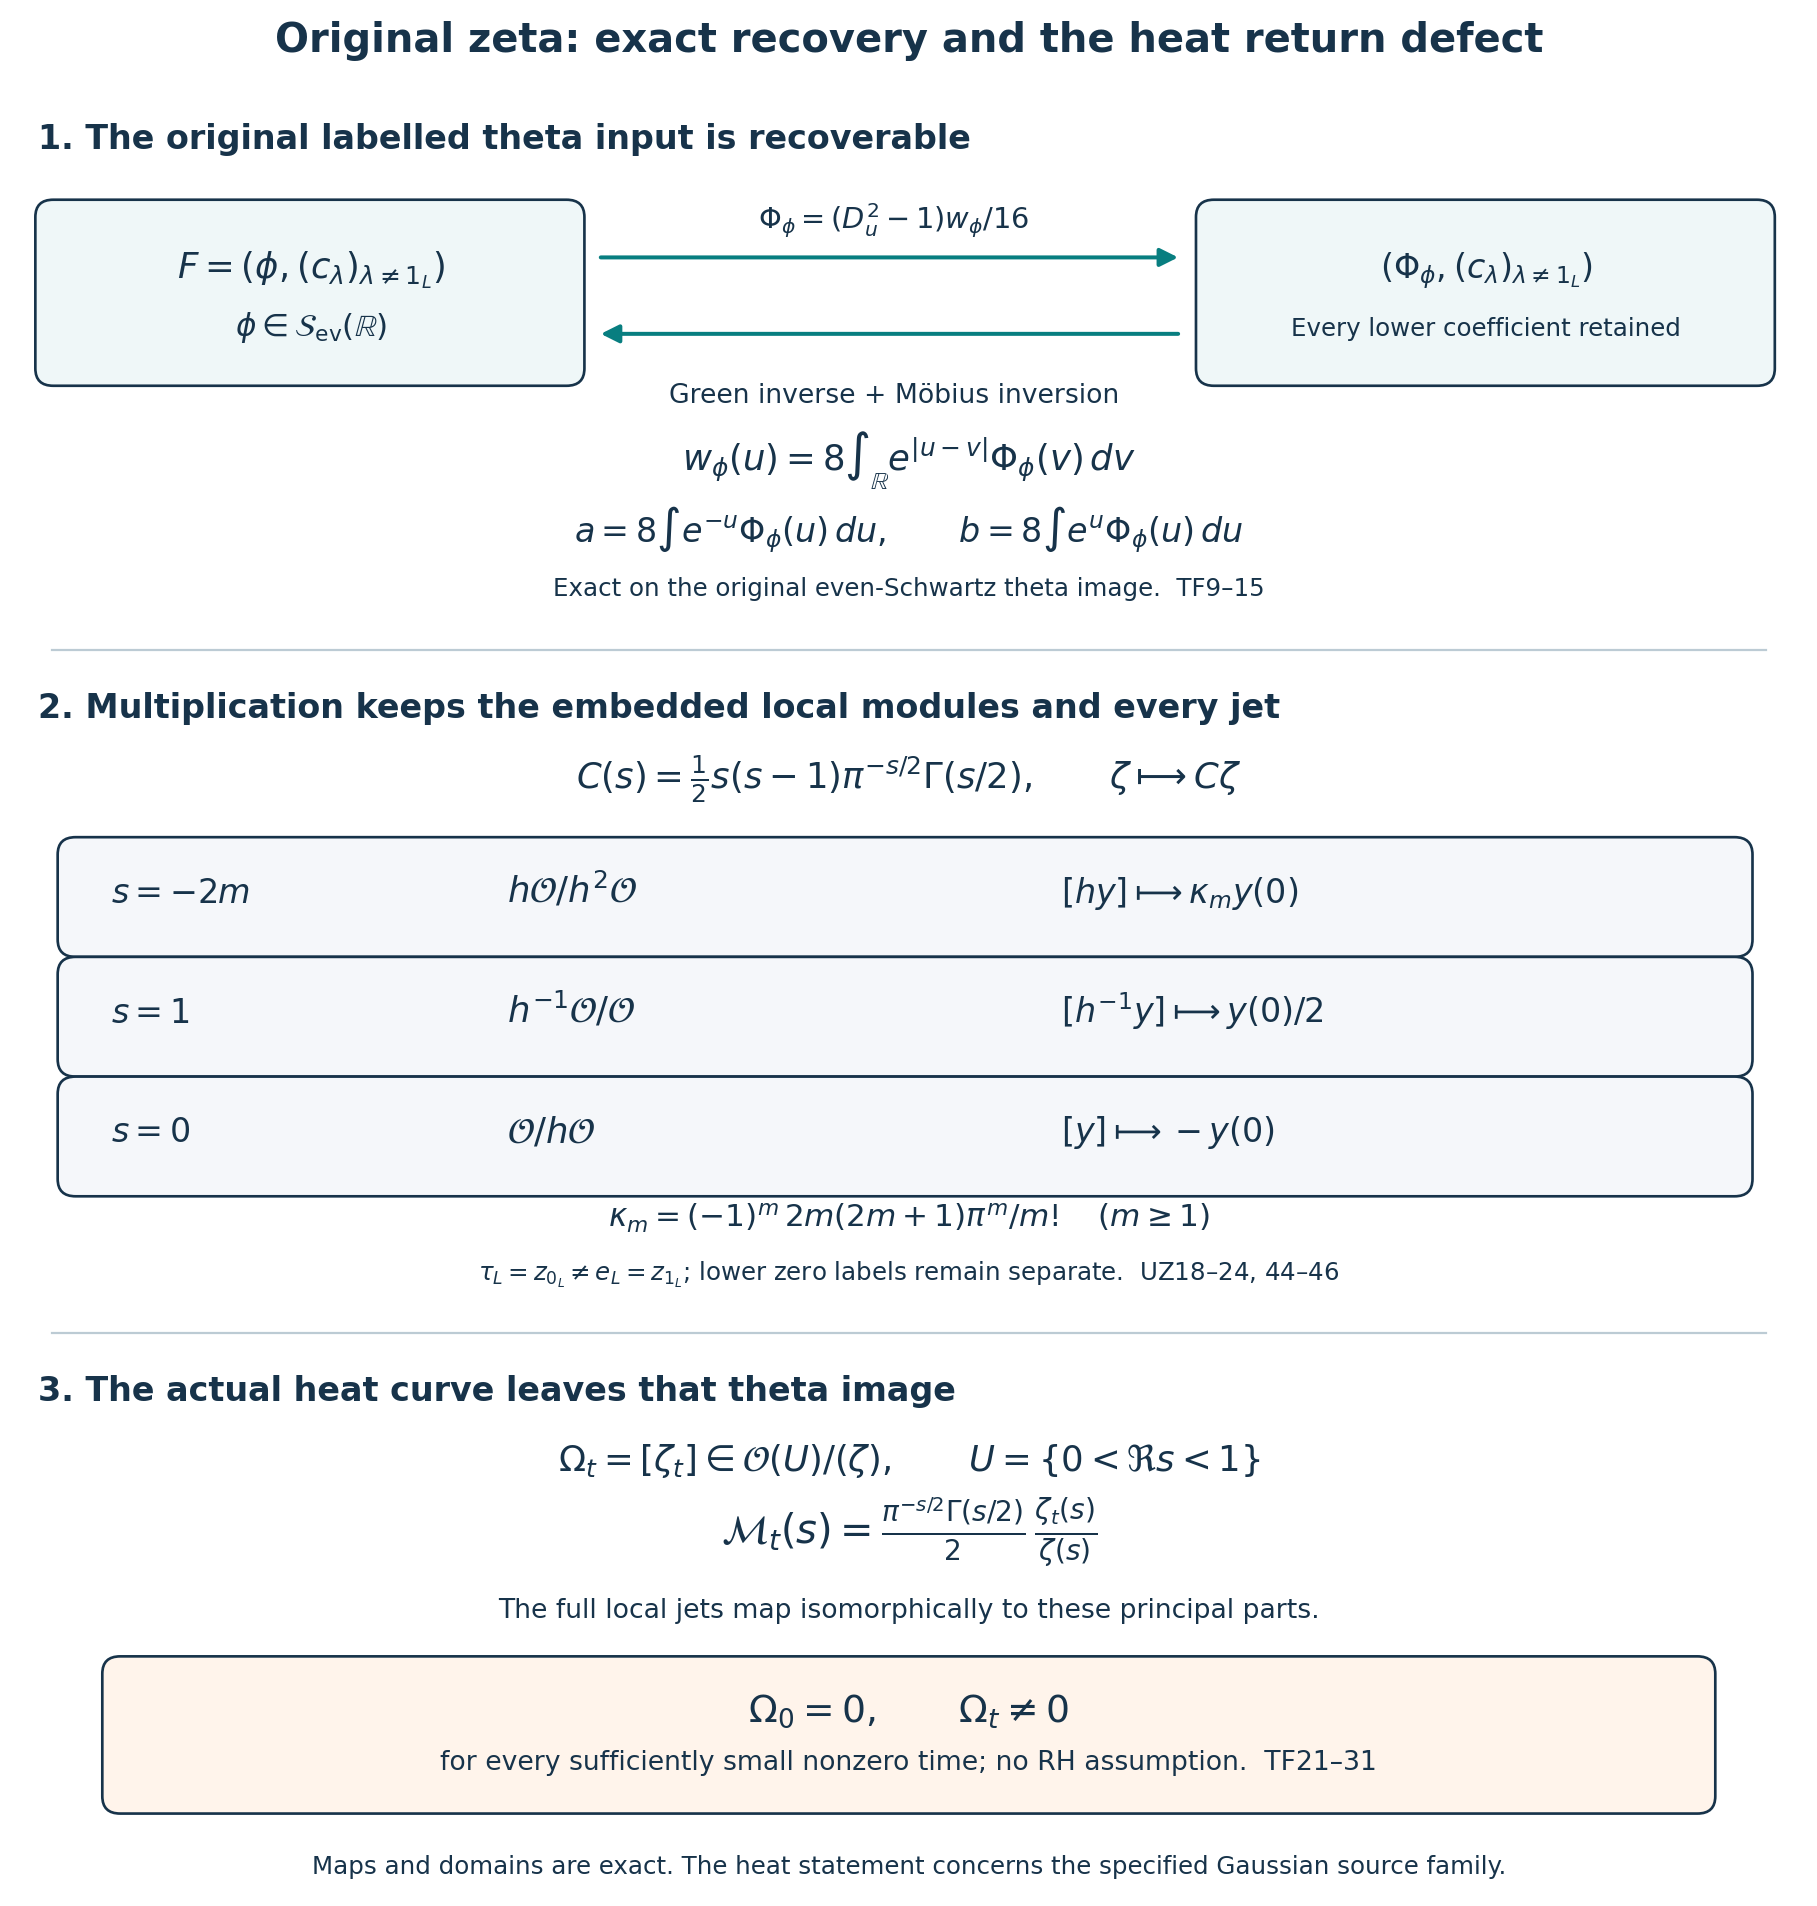
\includegraphics[keepaspectratio,alt={The exact original-zeta return. TF9--15 proves the filter and its inverse on the original even-Schwartz theta image, recovering both endpoints and every lower point-function coefficient. UZ18--24 and UZ44--46 prove the three embedded local fibre maps and retain all higher jets; h is the local coordinate s minus the point in each row. TF21--31 proves that the original Gaussian heat curve develops a nonzero return defect, and identifies its entire local jet tuple with the principal parts of the displayed meromorphic Mellin candidate. Its return obstruction is nonzero for every sufficiently small nonzero time. No zero location or RH assumption is used. Original heat convention: Rodgers--Tao, arXiv:1801.05914v5, equations hoz, phidef and htdef; every factor is retained in TF17--20.}]{faithful_theta_return.png}}
\caption{The exact original-zeta return. TF9--15 proves the filter and
its inverse on the original even-Schwartz theta image, recovering both
endpoints and every lower point-function coefficient. UZ18--24 and
UZ44--46 prove the three embedded local fibre maps and retain all higher
jets; h is the local coordinate s minus the point in each row. TF21--31
proves that the original Gaussian heat curve develops a nonzero return
defect, and identifies its entire local jet tuple with the principal
parts of the displayed meromorphic Mellin candidate. Its return
obstruction is nonzero for every sufficiently small nonzero time. No
zero location or RH assumption is used. Original heat convention:
Rodgers--Tao, arXiv:1801.05914v5, equations hoz, phidef and htdef; every
factor is retained in TF17--20.}
\end{figure}

\subsection{Original-zeta Gaussian and affine receiving
maps}\label{original-zeta-gaussian-and-affine-receiving-maps}

The complete extension OZG1--55 proves that Gaussian convolution of the
test at every positive time makes the original trivial-zero scalar sum
diverge for every real translation. Its admissible replacement retains
each cutoff trace and the Gamma boundary with the identical finite sum
U\_N; OZG20--27 gives both maps and the inverse. The full coefficient
tower, its raw non-Hermitian correction and exact compensated negative
index are OZG28--39. No compact-support prime window is assumed after
smoothing; all prime powers and Gamma terms, with explicit error bounds,
are OZG40--52. This extension acts on the tests while fixing the
original zeta zeros.

The different affine change of the actual original heat family is
OZR1--36. Its multiplier is exp(chi) C(phi)/C, with the full inverse,
exceptional units and local jets. The original generator contains every
q derivative term. The signed divisor comparison is OZR19--24; its
Cauchy logarithmic kernel has an additional growth contribution 2a.
OZR33 proves the exact full negative index after that contribution is
retained. The full support carrier and every lower coordinate are
OZG53--55 and OZR34--36. These are the receiving maps for these
specified extensions; the original preceding test, time and domains
remain those stated in its proof.

\end{document}
